\section{Results}

\subsection{Installation Status}
Both srsRAN Project and Open5GS were successfully installed on the SSH server.
The required dependencies and configurations were completed as part of the 
midterm milestone.

\subsection{UE Connection to gNB}
Figure \ref{fig:ue_connected} shows the UE successfully connected to the gNB.

\begin{figure}[h!]
    \centering
    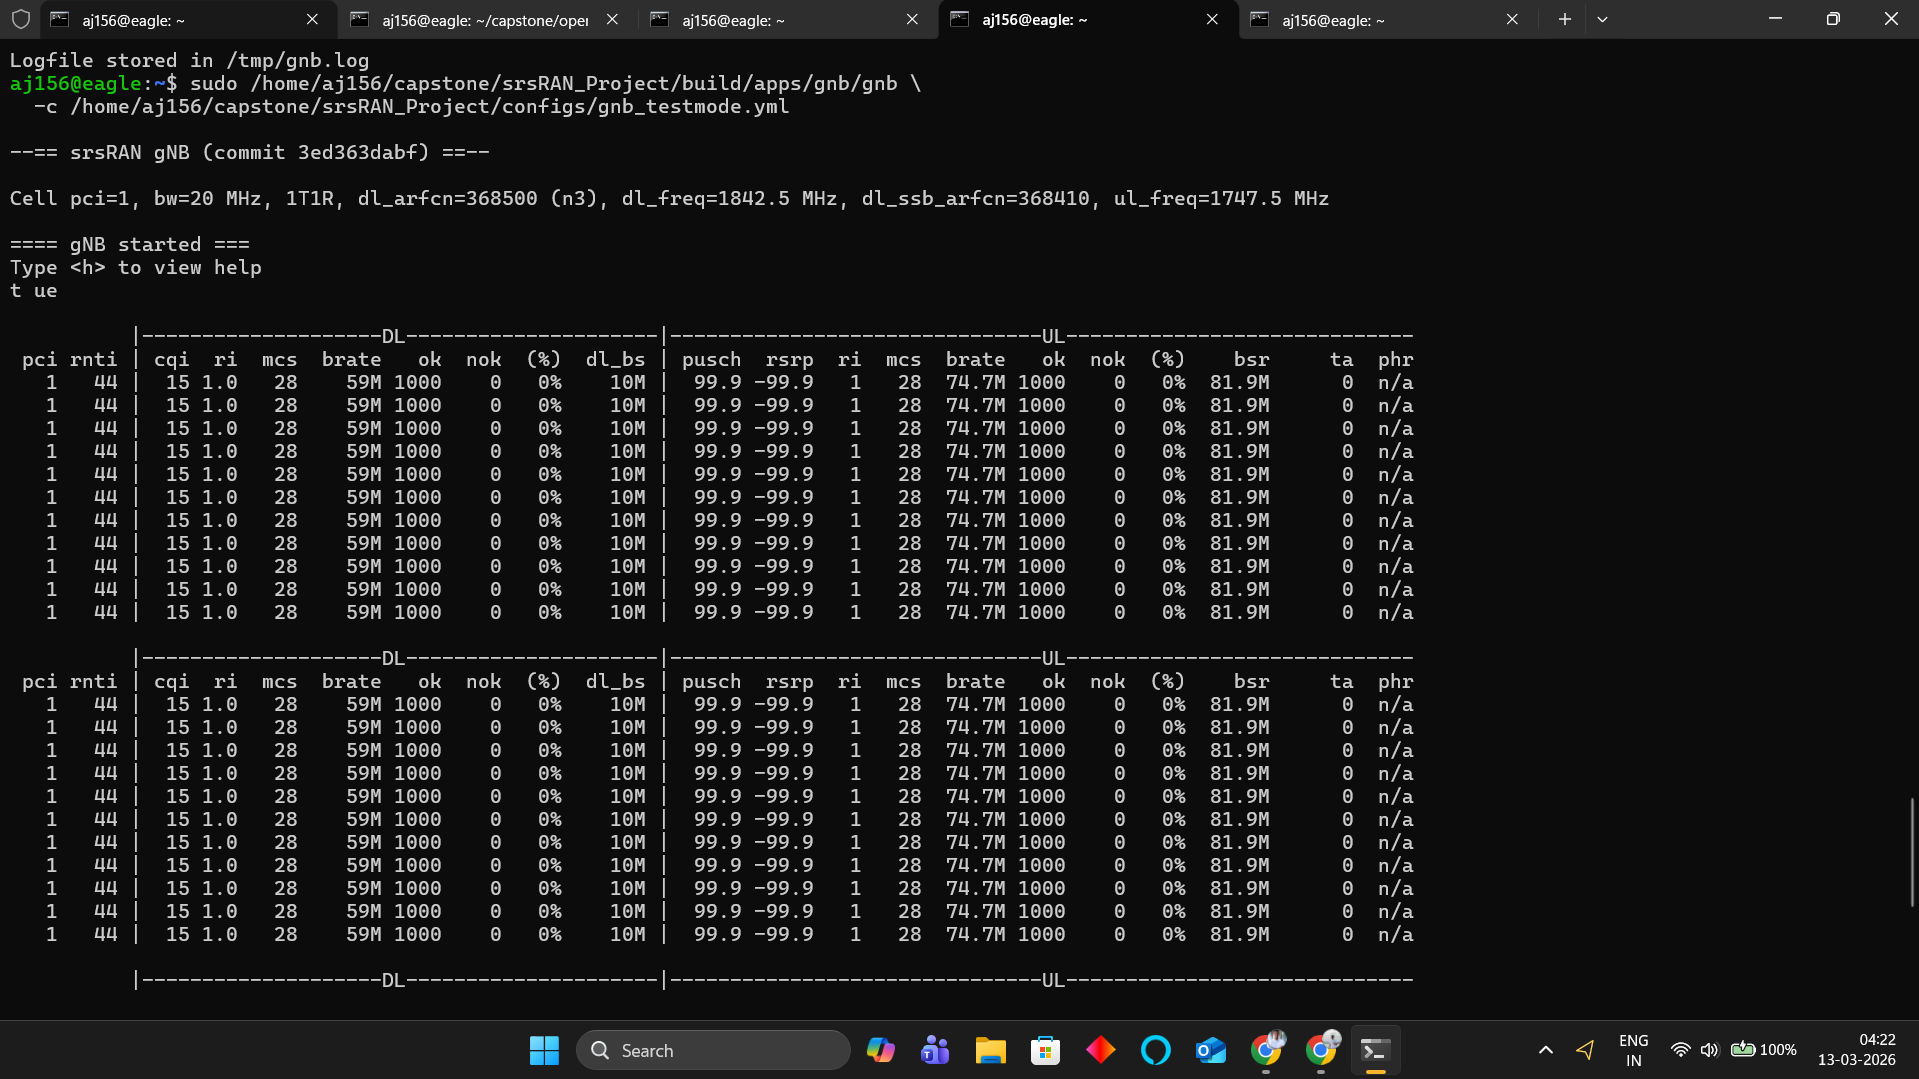
\includegraphics[width=0.9\textwidth]{figures/result1.png}
    \caption{UE Successfully Connected to gNB}
    \label{fig:ue_connected}
\end{figure}

\subsection{Uplink and Downlink Data}
Figure \ref{fig:uplink_downlink} shows the uplink and downlink data transmission.

\begin{figure}[h!]
    \centering
    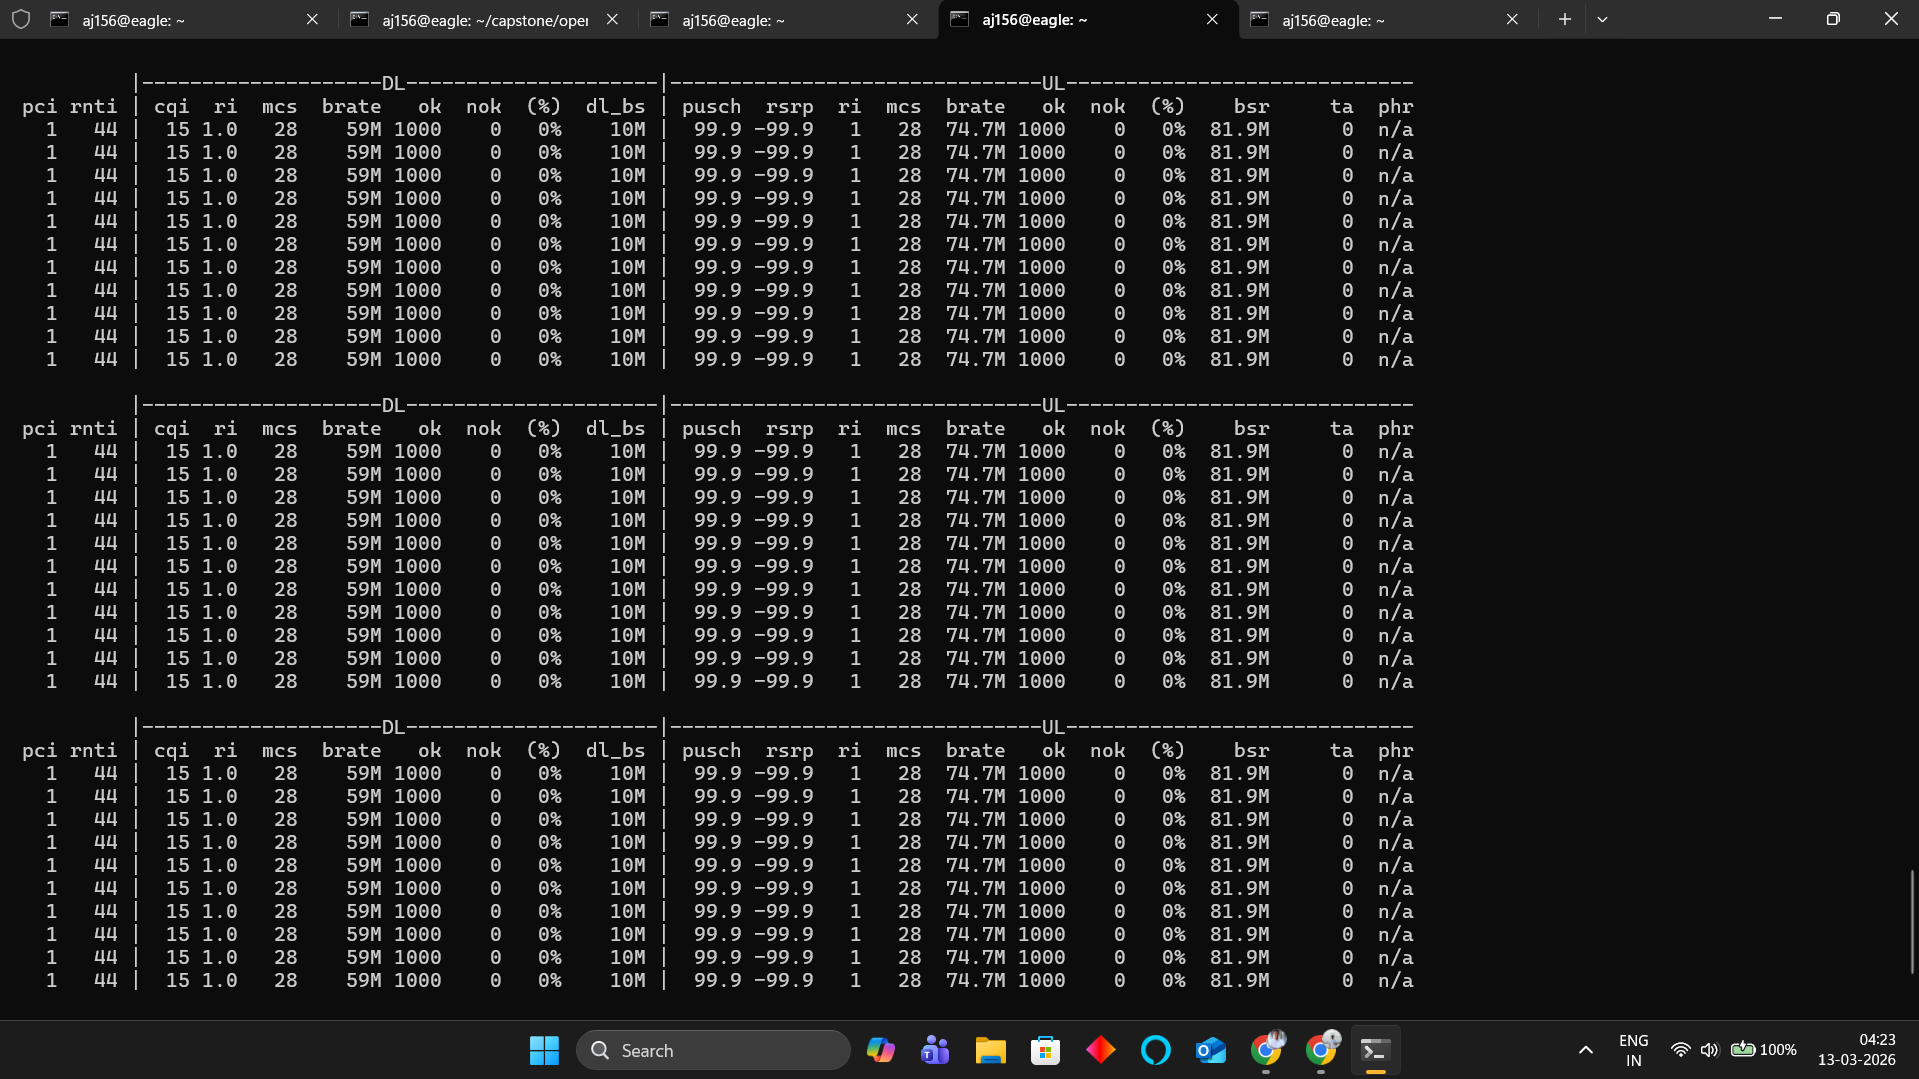
\includegraphics[width=0.9\textwidth]{figures/result2.png}
    \caption{Uplink and Downlink Data Transmission}
    \label{fig:uplink_downlink}
\end{figure}

\subsection{Configuration}
The following key configurations were applied:
\begin{itemize}
    \item Open5GS AMF configured with PLMN and slice information
    \item srsRAN gNB connected to Open5GS AMF via NGAP interface
    \item UE registration and authentication tested
\end{itemize}

\subsection{Current Progress}
\begin{itemize}
    \item[\checkmark] Open5GS installation complete
    \item[\checkmark] srsRAN Project installation complete
    \item[\checkmark] Basic configuration completed
    \item[\checkmark] UE connected to gNB
    \item[$\square$] Full end-to-end testing in progress
\end{itemize}

\subsection{Next Steps}
The remaining work includes completing end-to-end UE connectivity testing,
performance benchmarking, and analysis of the results using MATLAB.
```